% Options for packages loaded elsewhere
\PassOptionsToPackage{unicode}{hyperref}
\PassOptionsToPackage{hyphens}{url}
%
\documentclass[
]{article}
\usepackage{amsmath,amssymb}
\usepackage{lmodern}
\usepackage{iftex}
\ifPDFTeX
  \usepackage[T1]{fontenc}
  \usepackage[utf8]{inputenc}
  \usepackage{textcomp} % provide euro and other symbols
\else % if luatex or xetex
  \usepackage{unicode-math}
  \defaultfontfeatures{Scale=MatchLowercase}
  \defaultfontfeatures[\rmfamily]{Ligatures=TeX,Scale=1}
\fi
% Use upquote if available, for straight quotes in verbatim environments
\IfFileExists{upquote.sty}{\usepackage{upquote}}{}
\IfFileExists{microtype.sty}{% use microtype if available
  \usepackage[]{microtype}
  \UseMicrotypeSet[protrusion]{basicmath} % disable protrusion for tt fonts
}{}
\makeatletter
\@ifundefined{KOMAClassName}{% if non-KOMA class
  \IfFileExists{parskip.sty}{%
    \usepackage{parskip}
  }{% else
    \setlength{\parindent}{0pt}
    \setlength{\parskip}{6pt plus 2pt minus 1pt}}
}{% if KOMA class
  \KOMAoptions{parskip=half}}
\makeatother
\usepackage{xcolor}
\usepackage[margin=1in]{geometry}
\usepackage{graphicx}
\makeatletter
\def\maxwidth{\ifdim\Gin@nat@width>\linewidth\linewidth\else\Gin@nat@width\fi}
\def\maxheight{\ifdim\Gin@nat@height>\textheight\textheight\else\Gin@nat@height\fi}
\makeatother
% Scale images if necessary, so that they will not overflow the page
% margins by default, and it is still possible to overwrite the defaults
% using explicit options in \includegraphics[width, height, ...]{}
\setkeys{Gin}{width=\maxwidth,height=\maxheight,keepaspectratio}
% Set default figure placement to htbp
\makeatletter
\def\fps@figure{htbp}
\makeatother
\setlength{\emergencystretch}{3em} % prevent overfull lines
\providecommand{\tightlist}{%
  \setlength{\itemsep}{0pt}\setlength{\parskip}{0pt}}
\setcounter{secnumdepth}{-\maxdimen} % remove section numbering
\newlength{\cslhangindent}
\setlength{\cslhangindent}{1.5em}
\newlength{\csllabelwidth}
\setlength{\csllabelwidth}{3em}
\newlength{\cslentryspacingunit} % times entry-spacing
\setlength{\cslentryspacingunit}{\parskip}
\newenvironment{CSLReferences}[2] % #1 hanging-ident, #2 entry spacing
 {% don't indent paragraphs
  \setlength{\parindent}{0pt}
  % turn on hanging indent if param 1 is 1
  \ifodd #1
  \let\oldpar\par
  \def\par{\hangindent=\cslhangindent\oldpar}
  \fi
  % set entry spacing
  \setlength{\parskip}{#2\cslentryspacingunit}
 }%
 {}
\usepackage{calc}
\newcommand{\CSLBlock}[1]{#1\hfill\break}
\newcommand{\CSLLeftMargin}[1]{\parbox[t]{\csllabelwidth}{#1}}
\newcommand{\CSLRightInline}[1]{\parbox[t]{\linewidth - \csllabelwidth}{#1}\break}
\newcommand{\CSLIndent}[1]{\hspace{\cslhangindent}#1}
\usepackage{setspace}\doublespacing
\usepackage{lineno}\linenumbers
\usepackage{booktabs}
\usepackage{longtable}
\usepackage{array}
\usepackage{multirow}
\usepackage{wrapfig}
\usepackage{float}
\usepackage{colortbl}
\usepackage{pdflscape}
\usepackage{tabu}
\usepackage{threeparttable}
\usepackage{threeparttablex}
\usepackage[normalem]{ulem}
\usepackage{makecell}
\usepackage{xcolor}
\ifLuaTeX
  \usepackage{selnolig}  % disable illegal ligatures
\fi
\IfFileExists{bookmark.sty}{\usepackage{bookmark}}{\usepackage{hyperref}}
\IfFileExists{xurl.sty}{\usepackage{xurl}}{} % add URL line breaks if available
\urlstyle{same} % disable monospaced font for URLs
\hypersetup{
  pdftitle={XXX},
  hidelinks,
  pdfcreator={LaTeX via pandoc}}

\title{XXX}
\author{}
\date{\vspace{-2.5em}}

\begin{document}
\maketitle

\begin{center}
\textbf{H{\'{e}}ctor Tejero-Cicu{\'{e}}ndez$^{1,*}$,  Iris Men{\'{e}}ndez$^{2,3}$, Salvador Carranza$^{1}$, and Dean C. Adams$^{4}$} 
\end{center}

\begin{center}16 September, 2022\end{center}

\(^{1}\)Institute of Evolutionary Biology (CSIC-Universitat Pompeu
Fabra), Passeig Marítim de la Barceloneta 37-49, Barcelona 08002, Spain

\(^{2}\)Departamento de Geodinámica, Estratigrafía y Paleontología,
Facultad de Ciencias Geológicas, Universidad Complutense de Madrid,
C/José Antonio Novais 12, Madrid 28040, Spain

\(^{3}\)Departamento de Cambio Medioambiental, Instituto de Geociencias
(UCM, CSIC), C/Severo Ochoa 7, Madrid 28040, Spain

\(^{4}\)Department of Ecology, Evolution, and Organismal Biology, Iowa
State University, Ames, Iowa, 50010 USA

\(^{*}\)Correspondence: Héctor Tejero-Cicuéndez
\href{mailto:cicuendez93@gmail.com}{\nolinkurl{cicuendez93@gmail.com}}

\hfill\break

\textbf{Keywords}: Phenotypic Evolution, Morphospace, Allometry,
\emph{Pristurus} geckos \hfill\break

\textbf{Short Title}: XXX \hfill\break

\textbf{Author Contributions}: All authors collaboratively developed the
concept and contributed to all portions of this manuscript. HT-C, IM,
and DCA performed the analyses. All authors approve of the final product
and are willingly accountable for any portion of the
content.\hfill\break

\textbf{Conflicts of Interests}: The authors declare no conflicts of
interest.\hfill\break

\textbf{Data Archiving}: Data are available on DRYAD
(\url{doi:10.5061/dryad.xwdbrv1f6} (Tejero-Cicuéndez et al. 2021b)).
R-scripts are found in the Supplemental Information. \hfill\break

\textbf{Acknowledgments}: We thank XYZPDQ\ldots{} This work was
sponsored in part by XXX (to SC) DCA was funded in part by National
Science Foundation Grant DEB-2140720, and a Fulbright Senior Scholar
Grant.

\newpage

\hypertarget{abstract}{%
\section{Abstract}\label{abstract}}

asdf

\newpage

\hypertarget{introduction}{%
\section{Introduction}\label{introduction}}

some general paragraph on the evolution of phenotypic diversity
\hfill\break

when organisms colonize new and unique habitats, they are subjected to
novel ecological selection pressures in those habitats. Often these
selective pressures elicit changes in body form, as organisms adapt to
their new habitats (examples: some comment on ecomorphs, etc.). \ldots.
leads to so-called ecomorphs, with such well known examples in Anolis
lizards, cichlid fishes, etc. It follows that \ldots{} Some comment on
the fact that clades living in diverse ecological conditions often
display greater diversity in form and function (REFS).

However, while the above patterns have been well documented in a variety
of vertebrate taxa, what remains less known is how allometry plays a
role in this phenotypic diversification. We know that XYZPDQ (about
allometry). Then links to diversity..

The Afro-Arabian geckos in the genus \emph{Pristurus} afford the
opportunity to elucidate the interdigitating effects of allometry and
habitat specialization on clade-level patterns of phenotypic diversity.
Prior work on this system (Tejero-Cicuéndez et al. 2021a) has revealed
that \ldots{} (sentence or 2 about your prior study, getting to
diversity and \ldots{} Importantly, \ldots{} something about habitat.
\ldots. What remains unexamined however, is XYZPDQ\ldots{}

In this study, we \ldots{}

\hypertarget{materials-and-methods}{%
\section{Materials and Methods}\label{materials-and-methods}}

\hypertarget{data}{%
\subsection{Data}\label{data}}

Phylogenetic, ecological, phenotypic\ldots. (describe briefly). Data
from (Tejero-Cicuéndez et al. 2021a).

\hypertarget{statistical-analyses}{%
\subsection{Statistical Analyses}\label{statistical-analyses}}

To test the hypothesis\ldots{}

\begin{itemize}
\tightlist
\item
  Mancova body \textasciitilde{} SVL*hab.gp

  \begin{itemize}
  \tightlist
  \item
    PW of slopes, and inspected reg. coefficients to identify biological
    trends
  \item
    Visualized multivariate regressions via regression scores (sensu
    Drake and Klingenberg 2008) and predicted lines (sensu Adams and
    Nistri 2010)
  \end{itemize}
\item
  Examine allometry phylogenetically.

  \begin{itemize}
  \tightlist
  \item
    PLS of head vs.~SVL and limb vs SVL. Obtained scores on 1st axis for
    each.
  \item
    within-species regressions of Head.sc \textasciitilde{} SVL \&
    limb.sc \textasciitilde{} SVL; obtained regression coefficients
    (slopes)
  \item
    mapped slopes on phylogeny under BM and generated traitgrams to
    identify changes in allometric relationships across the phylogeny
  \end{itemize}
\item
  Finally, to link allometric patterns with trends in phenotypic
  diversification we obtained size-standardized species means, following
  procedures in H TC paper (residuals from phylo-regressions of traits
  on SVL, residuals). We then performed an ordination to obtain a
  phylomorphospace, where habitat types and species could be observed.
\end{itemize}

\hypertarget{results}{%
\section{Results}\label{results}}

\hypertarget{discussion}{%
\section{Discussion}\label{discussion}}

\newpage

\hypertarget{references}{%
\section*{References}\label{references}}
\addcontentsline{toc}{section}{References}

\setlength{\parindent}{-0.25in} \setlength{\leftskip}{0.25in}
\setlength{\parskip}{8pt} \noindent

\hypertarget{refs}{}
\begin{CSLReferences}{1}{0}
\leavevmode\vadjust pre{\hypertarget{ref-AdamsNistri2010}{}}%
Adams, D. C., and A. Nistri. 2010. Ontogenetic convergence and evolution
of foot morphology in european cave salamanders (family:
plethodontidae). BMC Evolutionary Biology 10:1--10. BioMed Central.

\leavevmode\vadjust pre{\hypertarget{ref-DrakeKlingenberg2008}{}}%
Drake, A. G., and C. P. Klingenberg. 2008.
\href{https://doi.org/10.1098/rspb.2007.1169}{The pace of morphological
change: Historical transformation of skull shape in st bernard dogs}.
Proceedings of the Royal Society B: Biological Sciences 275:71--76.

\leavevmode\vadjust pre{\hypertarget{ref-Tejero-Cicuendez2021}{}}%
Tejero-Cicuéndez, H., M. Simó-Riudalbas, I. Menéndez, and S. Carranza.
2021a. \href{https://doi.org/10.1098/rspb.2021.1821}{Ecological
specialization, rather than the island effect, explains morphological
diversification in an ancient radiation of geckos}. Proceedings of the
Royal Society B: Biological Sciences 288:20211821.

\leavevmode\vadjust pre{\hypertarget{ref-PristurusData}{}}%
Tejero-Cicuéndez, H., M. Simó-Riudalbas, I. Menéndez, and S. Carranza.
2021b. Ecological specialization, rather than the island effect,
explains morphological diversification in an ancient radiation of
geckos. Dryad digital repository. (Doi:10.5061/dryad.xwdbrv1f6).

\end{CSLReferences}

\newpage

\hypertarget{figures}{%
\section{Figures}\label{figures}}

Figure 1. Linear Measures \hfill\break

Figure 2. Plot of regression scores and predicted lines representing the
relationship between linear body measurements and size (SVL).
Individuals occupying differing habitats are denoted by distinct colors
as: rock (beige), ground (dark purple), and tree (magenta). \hfill\break

Figure 3. Traitgrams showing the evolution of body size (SVL) through
time mapped on the phylogenetic tree of \emph{Pristurus}. Colors
represent evolutionary mapping of

colored by (A) mapped by the discrete categories of presence in Socotra
or the continent (left) and by ecological specialization (right).
\hfill\break

Figure 4. Phylomorphospace

\newpage

\begin{figure}[H]

\includegraphics[width=1\linewidth]{Figs/Fig1} \caption{asdf.}\label{fig:unnamed-chunk-1}
\end{figure}

\newpage

\begin{figure}[H]
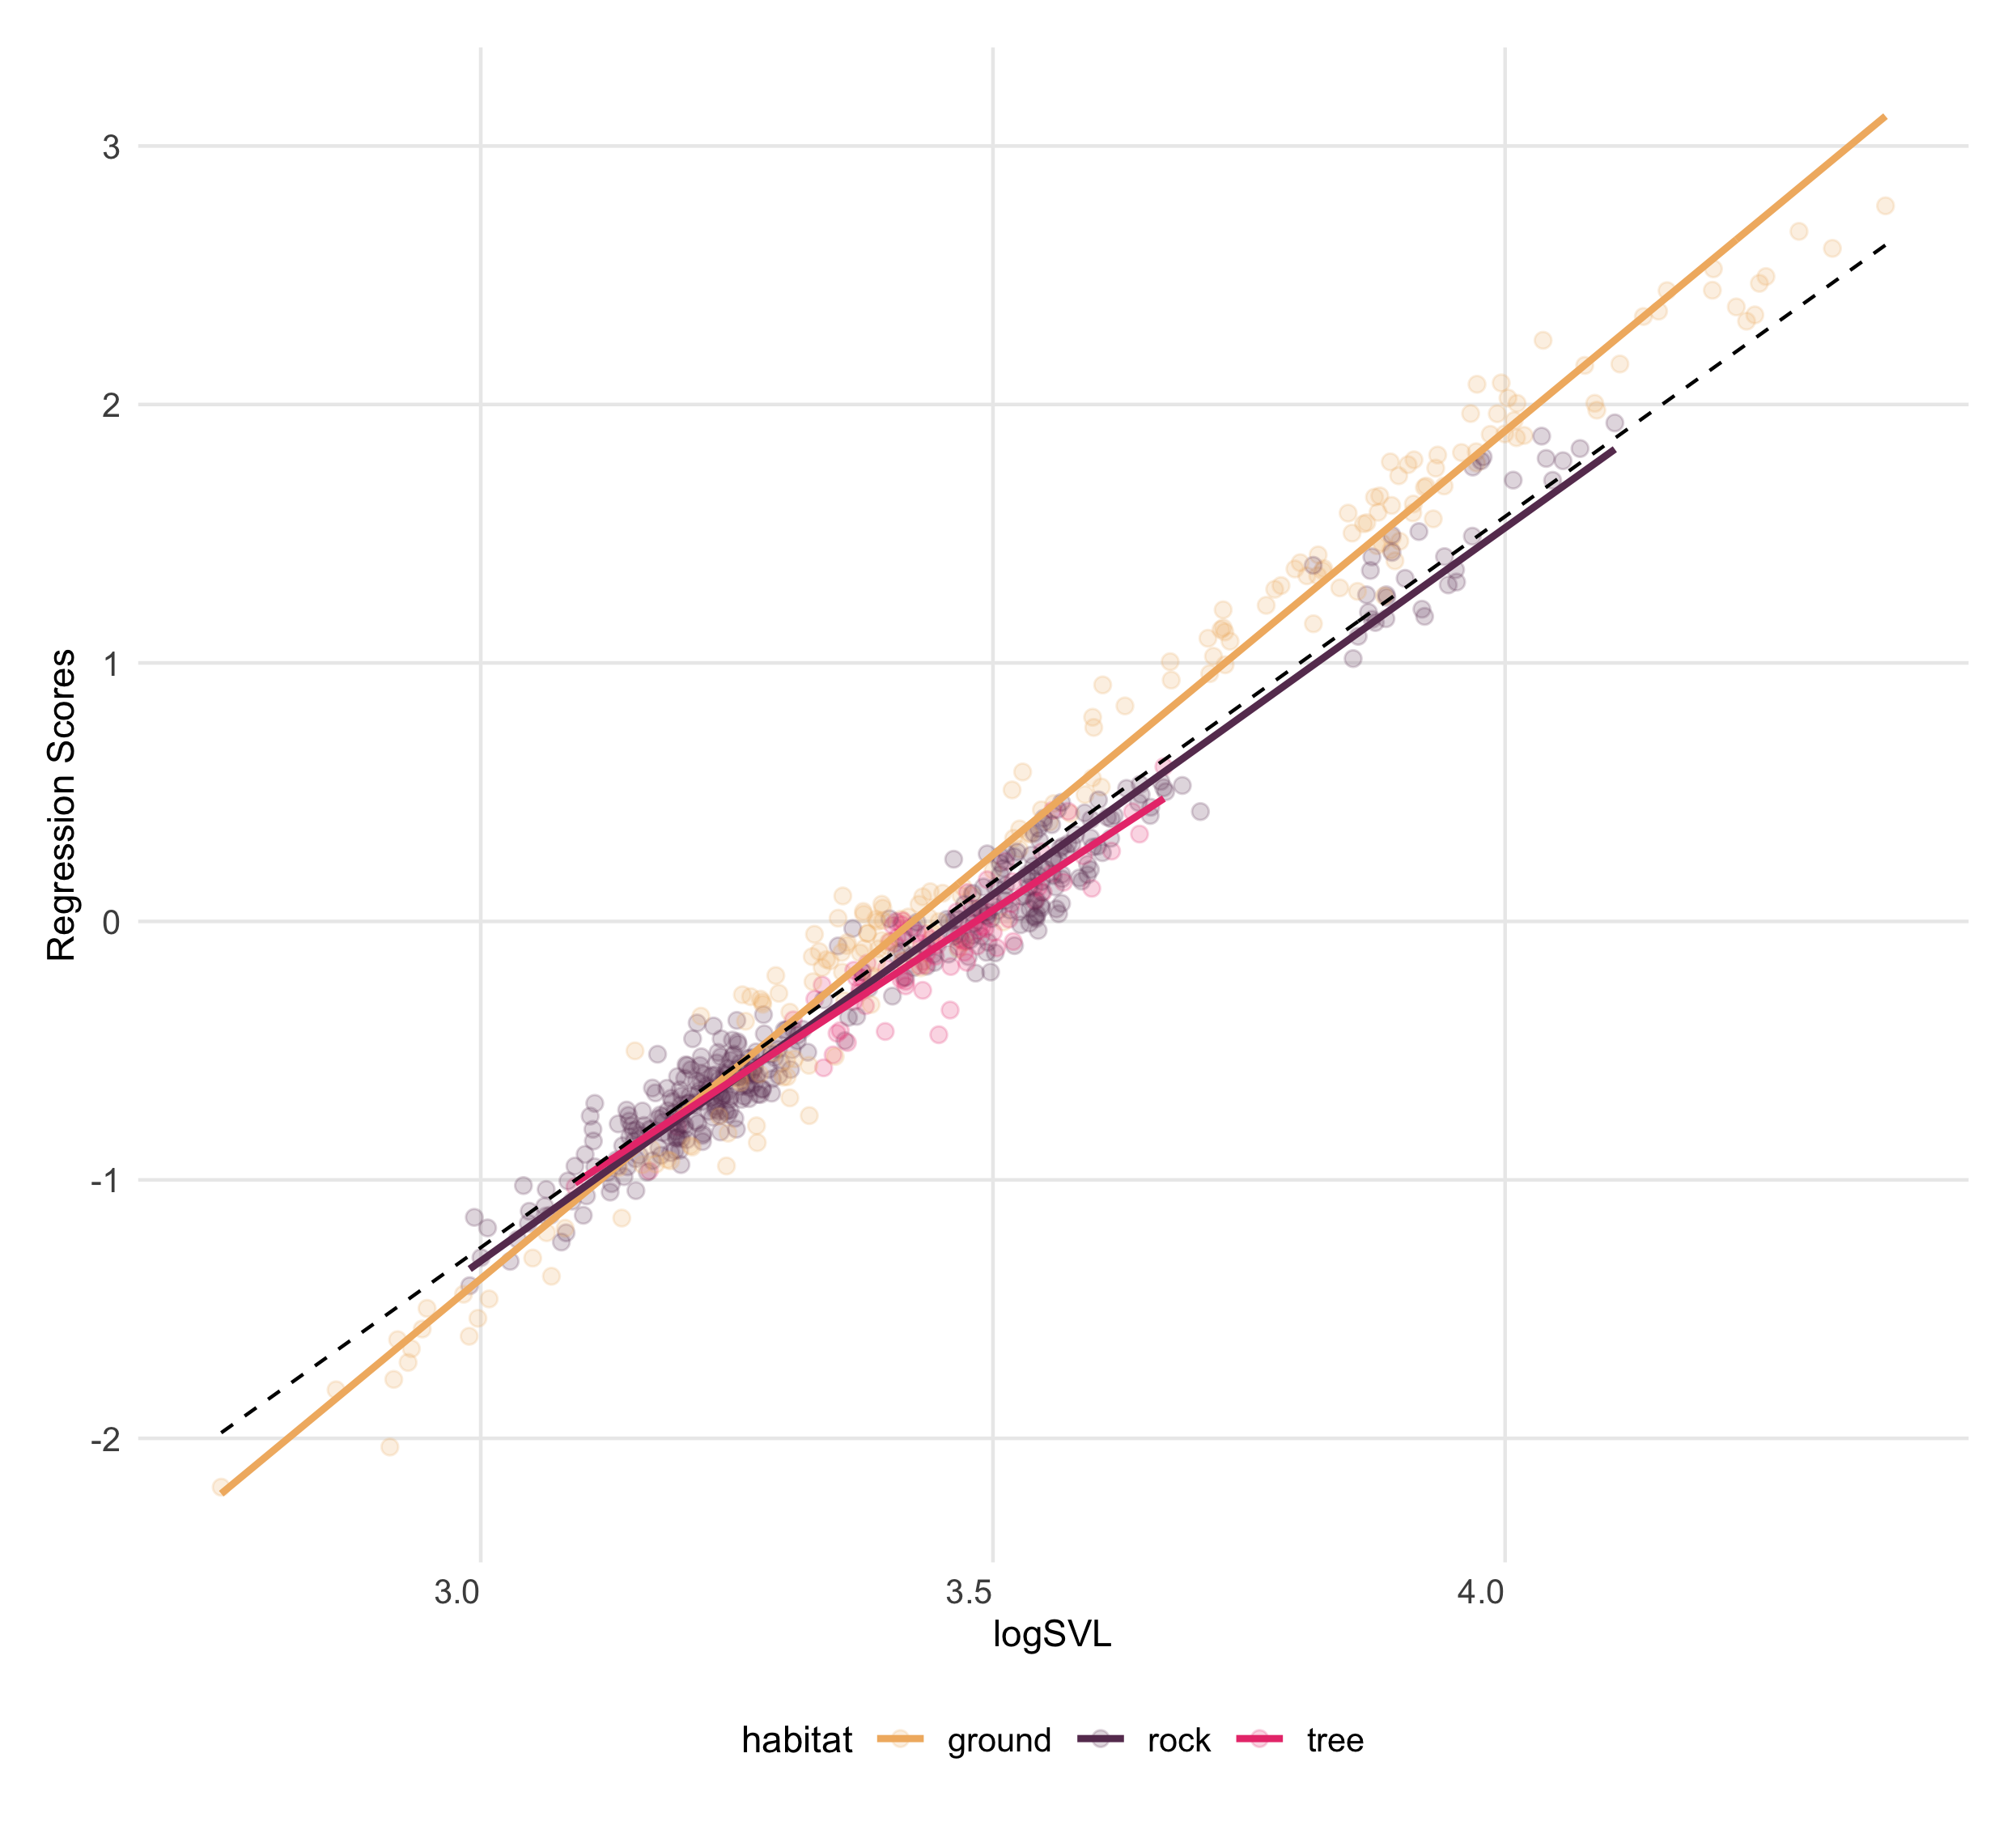
\includegraphics[width=1\linewidth]{Figs/figure_2_ggplot} \caption{Plot of regression scores and predicted lines representing the relationship body proportions and body size (SVL). Individuals occupying differing habitats are denoted by distinct colors as: rock (beige), ground (dark purple), and tree (magenta).}\label{fig:unnamed-chunk-2}
\end{figure}

\newpage

\begin{figure}
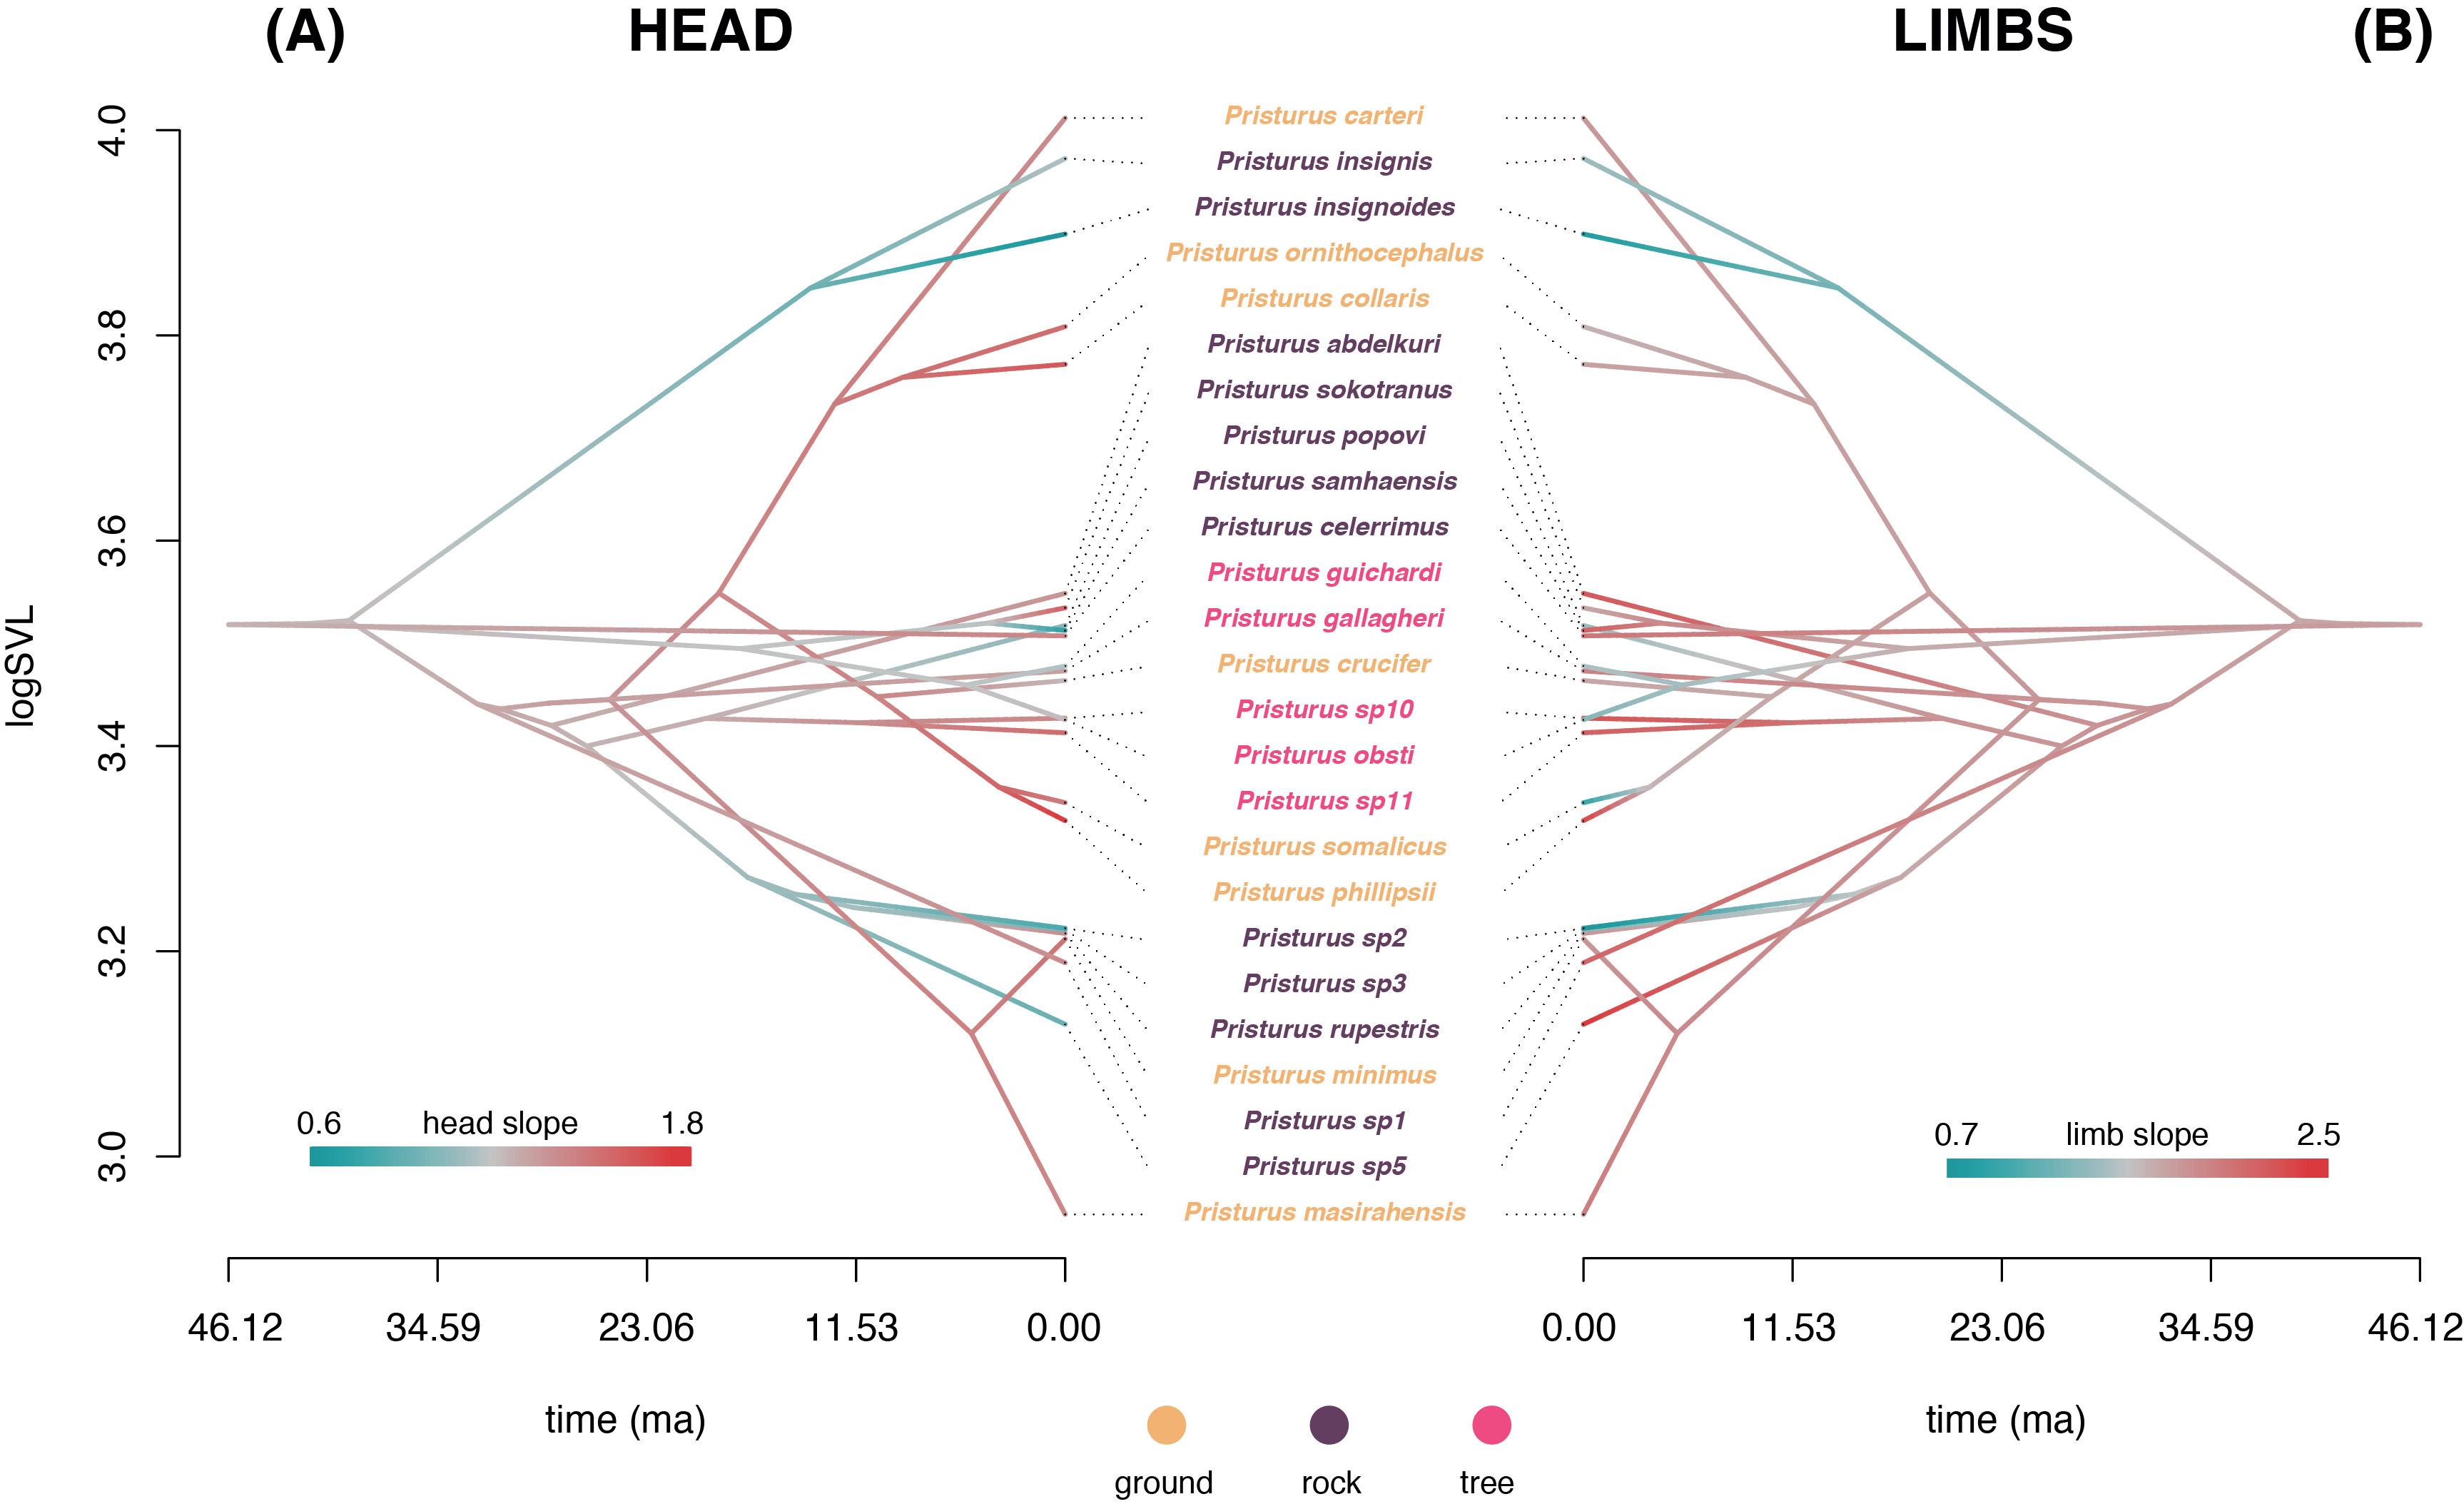
\includegraphics[width=1\linewidth]{Figs/figure_phenograms} \caption{xxx.}\label{fig:unnamed-chunk-3}
\end{figure}

\newpage

\begin{figure}
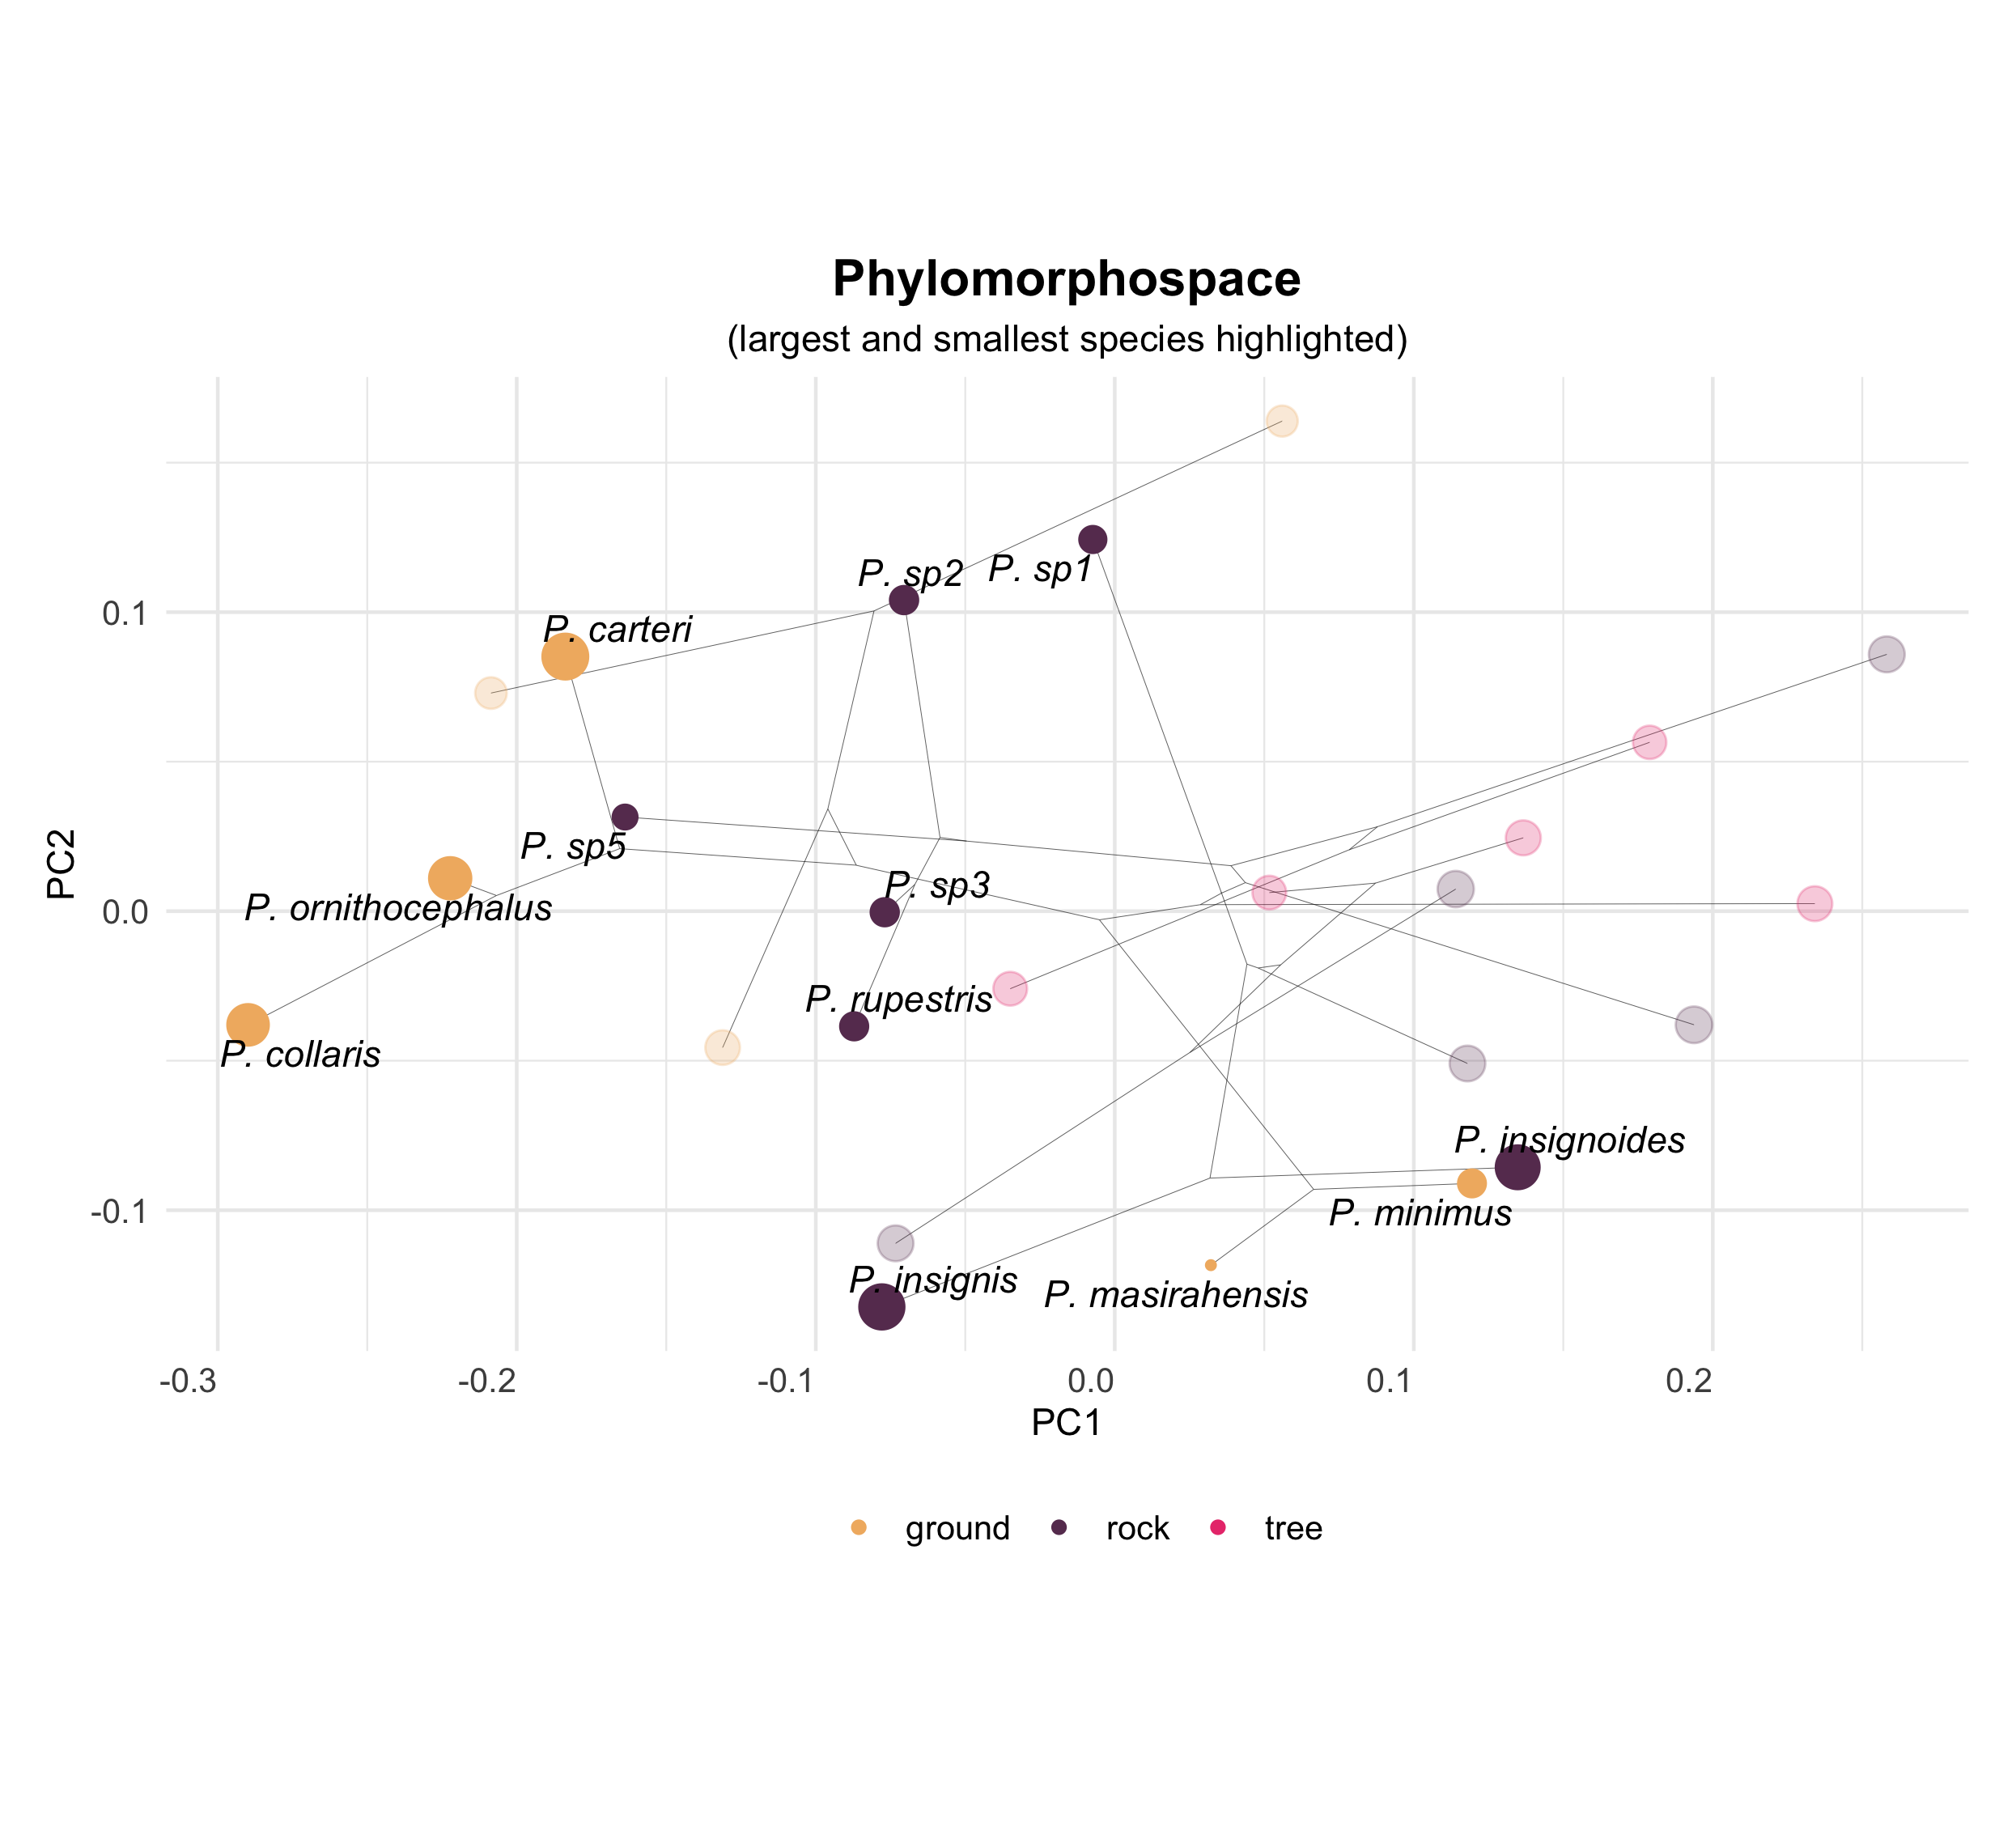
\includegraphics[width=1\linewidth]{Figs/phylomorphospace_large_small} \caption{asdf.}\label{fig:unnamed-chunk-4}
\end{figure}

\end{document}
